\chapter{The p-Block II: Oxygen, Halogens and Noble Gases}\label{ch:b1:p-block-16-18}

Sulfuric acid is made in larger tonnage than any other chemical: it
dissolves phosphate rock for fertilisers, leaches copper and uranium ores,
refines oil and fills car batteries, and for a century the output of
sulfuric acid was a rough measure of a country's industry. Most of its
sulfur now comes from the cleaning of natural gas and oil; some is still
carried by hand out of volcanic craters. Sulfur sits in \omterm{def:b1:periodicity:table}{group} 16 under
oxygen; the \omterm{def:b1:p-block-16-18:halogen}{halogens} of \omterm{def:b1:periodicity:table}{group} 17 and the noble gases of \omterm{def:b1:periodicity:table}{group} 18 complete
the \omterm{def:b1:periodicity:table}{p-block}. This chapter follows oxygen and sulfur from the element to
the acid, ranks the \omterm{def:b1:p-block-16-18:halogen}{halogens} as \omterm{def:b1:nernst:couple}{oxidants} with their \omterm{def:b1:nernst:electrode-potential}{standard potentials},
and ends with the compounds that the supposedly inert noble gases do form.

\begin{recall}
\omterm{def:b1:lewis-resonance-vsepr:lewis}{Lewis structures}, expanded octets and the VSEPR shapes (\cref{ch:b1:lewis-resonance-vsepr});
\omterm{def:b1:nernst:electrode-potential}{standard potentials} (\cref{ch:b1:nernst}); the \omterm{def:b1:e-ph-diagrams:disproportionation}{disproportionation} of
chlorine and the \omterm{def:b1:e-ph-diagrams:e-ph-diagram}{potential--pH diagram} of chlorine
(\cref{ch:b1:e-ph-diagrams}); catalysis (\cref{ch:b1:elementary-steps}).
The school volume (grade 10) grouped the \omterm{def:b1:p-block-16-18:halogen}{halogens} and noble gases as
families.
\end{recall}

\begin{omfigure}
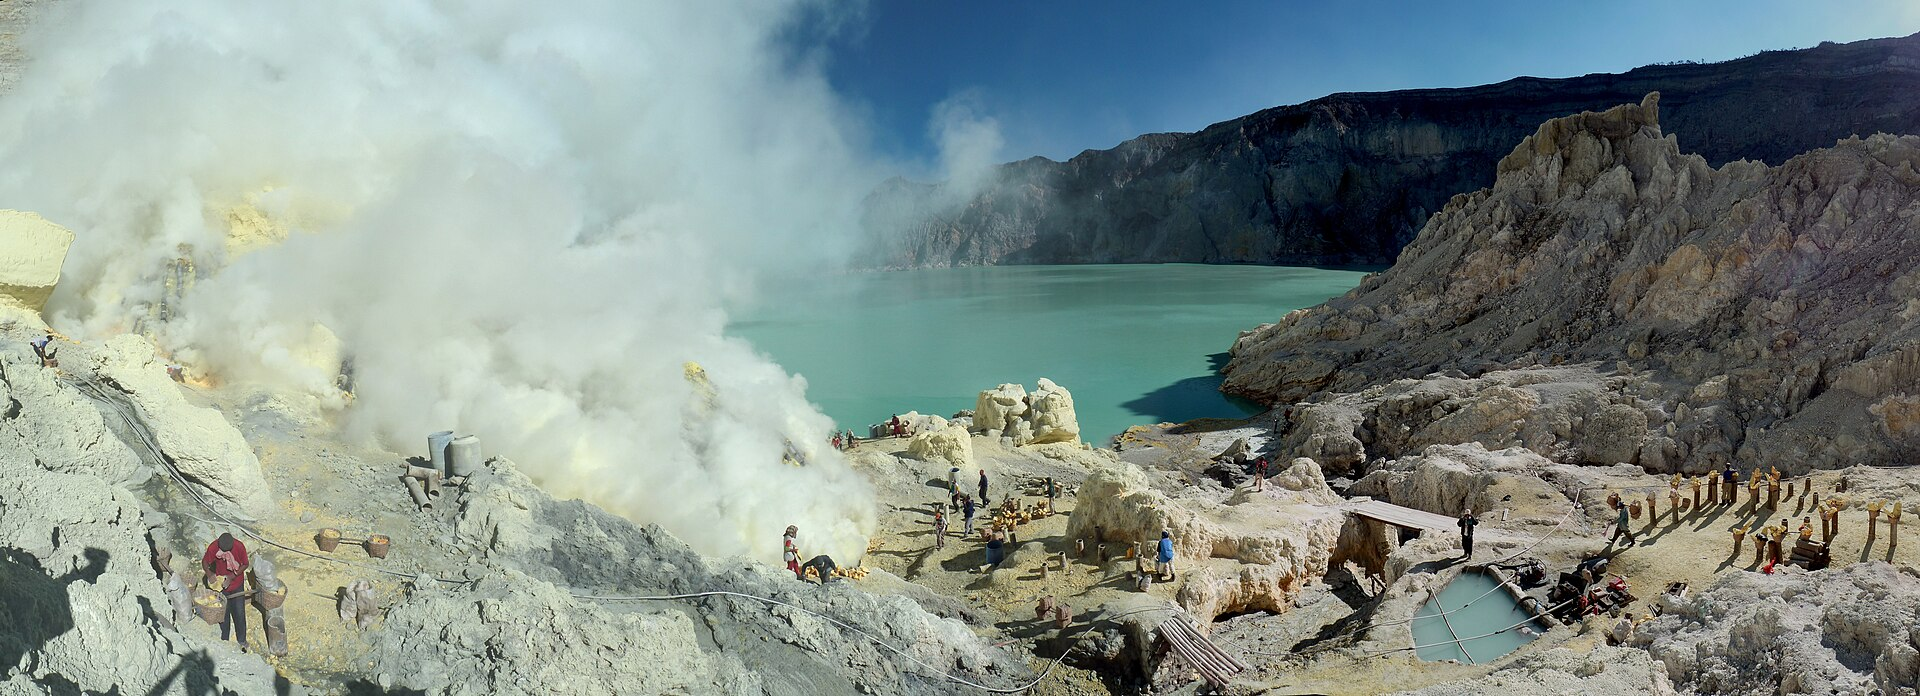
\includegraphics[width=0.78\linewidth]{images/book2/kawah-ijen.jpg}

{\small Sulfur mining in the crater of the Kawah Ijen volcano, Indonesia:
volcanic gases condense yellow sulfur around pipes, and miners carry it
out in baskets (photograph Sémhur, CC BY-SA 4.0, Wikimedia Commons).}
\end{omfigure}

\section{Oxygen, ozone and peroxides}

\begin{definition}[Chalcogens]\label{def:b1:p-block-16-18:chalcogen}
The \emph{chalcogens}\index{chalcogen} are the elements of \omterm{def:b1:periodicity:table}{group} 16
(O, S, Se, Te, Po), with six \omterm{def:b1:quantum-numbers:configuration}{valence electrons} \textit{ns}$^2$\textit{np}$^4$.
They form compounds with \omterm{def:b1:nernst:oxidation-number}{oxidation numbers} from $-$II (oxides, sulfides)
to $+$VI (sulfates), the higher ones only for sulfur and below.
\end{definition}

Oxygen exists as dioxygen \ce{O2} and as ozone \ce{O3}, a bent molecule
with two \omterm{def:b1:lewis-resonance-vsepr:resonance}{resonance structures} (\cref{ch:b1:lewis-resonance-vsepr}). Ozone
is a stronger \omterm{def:b1:nernst:couple}{oxidant} than dioxygen: $E^\circ(\ce{O3}/\ce{O2}) = 2.07$~V
against 1.23~V for \ce{O2}/\ce{H2O}. In the upper atmosphere it absorbs
ultraviolet light; near the ground it is a pollutant. Hydrogen peroxide,
with an \ce{O-O} bond and oxygen at $-$I, is both \omterm{def:b1:nernst:couple}{oxidant} and \omterm{def:b1:nernst:couple}{reductant}
and disproportionates slowly (\cref{exo:b1:nernst:12}).
% ledger: dfg:O3_g (E0 computed in figdata/bachelor-1/standard-potentials.py)

\begin{example}[The oxidation numbers of oxygen]
Oxygen, second only to fluorine in \omterm{def:b1:periodicity:electronegativity}{electronegativity}, is at $-$II in
almost all its compounds: water, oxides, hydroxides, sulfates. The
exceptions follow from the rule that the shared electrons go to the more
electronegative partner and are split equally between identical atoms. In
hydrogen peroxide \ce{H2O2}, H--O--O--H, each oxygen takes the electrons of
its \ce{O-H} bond but shares the \ce{O-O} pair: $-$I. In potassium
superoxide \ce{KO2}, the ion \ce{O2-} carries one charge for two atoms:
$-\frac12$ on average. In oxygen difluoride \ce{OF2}, fluorine wins both
bonds and oxygen is at $+$II. In \ce{O2} and \ce{O3} it is at 0. Only the
$-$II state is stable towards water; peroxides and superoxides are
\omterm{def:b1:nernst:couple}{oxidants}, and \ce{OF2} a fluorinating agent.
\end{example}

\section{Sulfur and sulfuric acid}

Sulfur, unlike oxygen, forms rings and chains of single \ce{S-S} bonds:
ordinary sulfur is made of \ce{S8} rings. It burns to sulfur dioxide, a
bent molecule (O--S--O angle \ang{119.5}), which can be oxidised further
to sulfur trioxide, trigonal planar. Both are \omterm{def:b1:s-block:oxide-character}{acidic oxides}: \ce{SO2}
gives sulfurous acid ($\mathrm{p}K_a$ 1.77 and 7.22), \ce{SO3} sulfuric
acid.
% ledger: geo:SO2.aOSO, dfg:SO2_g, dfg:SO3_g

\begin{proposition}[Steps of the contact process]\label{prop:b1:p-block-16-18:contact-steps}
Sulfuric acid is made from sulfur in four steps:
(1) \ce{S + O2 -> SO2}; (2) \ce{2SO2 + O2 <=> 2SO3}, over a vanadium(V)
oxide \omterm{def:b1:elementary-steps:catalyst}{catalyst}; (3) \ce{SO3 + H2SO4 -> H2S2O7} (oleum), the trioxide being
absorbed in concentrated acid; (4) \ce{H2S2O7 + H2O -> 2H2SO4}. Overall,
\ce{2S + 3O2 + 2H2O -> 2H2SO4}.
\end{proposition}

\begin{proof}
Each step is balanced; adding $2\times(1)$, (2), $2\times(3)$ and
$2\times(4)$, the \ce{SO2}, \ce{SO3} and \ce{H2S2O7} cancel, and the two
\ce{H2SO4} consumed in step 3 are regenerated in step 4, which leaves
\ce{2S + 3O2 + 2H2O -> 2H2SO4}. Step 2 is thermodynamically very
favourable at room temperature ($K = 10^{24.8}$ at \qty{25}{\celsius}, from
the Gibbs energies of formation) but extremely slow: the \omterm{def:b1:elementary-steps:catalyst}{catalyst}, active
only when hot, is what makes it run, and the compromise between rate and
conversion is studied in the Year~2 volume. \ce{SO3} is not absorbed in
water directly, because its reaction with water vapour forms a fine mist
of acid droplets that passes through the absorbers.
\end{proof}
% ledger: dfg:SO2_g, dfg:SO3_g

\begin{omfigure}
\begin{tikzpicture}[font=\small, >={Stealth}, box/.style={draw, rounded corners, fill=omDef!8, align=center, minimum height=1.0cm}]
  \node[box] (b) at (0,0) {sulfur burner\\\ce{S + O2 -> SO2}};
  \node[box] (c) at (4.4,0) {converter, \ce{V2O5}\\catalyst beds};
  \node[box] (a) at (8.8,0) {absorption tower\\\ce{SO3} into \ce{H2SO4}};
  \node[box] (d) at (8.8,-2.2) {dilution\\\ce{H2S2O7 + H2O}};
  \draw[<-, thick] (b.west) -- ++(-0.8,0) node[left] {air, S};
  \draw[->, thick] (b) -- node[above] {\ce{SO2}} (c);
  \draw[->, thick] (c) -- node[above] {\ce{SO3}} (a);
  \draw[->, thick] (a) -- node[right] {oleum} (d);
  \draw[->, thick] (d.west) -- ++(-1.2,0) node[left] {\ce{H2SO4}};
  \draw[->, thick] (d.east) -- ++(0.6,0) |- node[pos=0.25, right] {part returned} (a.east);
\end{tikzpicture}

{\small The contact process: burning sulfur, catalytic oxidation of
\ce{SO2}, absorption of \ce{SO3} in concentrated sulfuric acid, and
dilution of the oleum. Part of the acid is returned to the absorber.}
\end{omfigure}

\begin{proposition}[Strength of sulfuric acid]\label{prop:b1:p-block-16-18:sulfuric-strength}
In water, the first acidity of sulfuric acid is strong (total), the
second weak: $\mathrm{p}K_a(\ce{HSO4-}/\ce{SO4^2-}) = 1.99$. A
\qty{0.010}{mol/L} solution is therefore not at pH 1.70 (two protons) nor
at 2.00 (one), but in between.
\end{proposition}

\begin{proof}
\ce{H2SO4}, with two oxygens without hydrogen on sulfur, is an \omterm{def:b1:p-block-13-15:oxoacid}{oxoacid}
stronger than \ce{H3O+}: levelled (\cref{ch:b1:predominant-reaction}).
\ce{HSO4-}, already negative, holds its proton more: its $\mathrm{p}K_a$,
computed from the Gibbs energies of formation, is 1.99. At $C = 0.010$:
$[\ce{H3O+}] = C + x$, $[\ce{HSO4-}] = C - x$, $[\ce{SO4^2-}] = x$, with
$x(C + x)/(C - x) = 10^{-1.99}$; solving, $x = \qty{4.2e-3}{mol/L}$ and
$\mathrm{pH} = -\log(0.0142) = 1.85$.
\end{proof}
% ledger: dfg:HSO4-_ao, dfg:SO42-_ao

Concentrated sulfuric acid is also a powerful dehydrating agent (it chars
sugar, taking the elements of water from it) and, hot, an \omterm{def:b1:nernst:couple}{oxidant}. Diluting
it releases much heat: the acid is always poured into the water, never the
reverse. Most of the world's sulfur, about 84 million tonnes in 2025, is
recovered from the hydrogen sulfide of natural gas and refinery streams,
and most of it ends as sulfuric acid.
% ledger: usgs:S-world-2025

\begin{method}[Mass balance through the contact process]\label{met:b1:p-block-16-18:contact-balance}
\begin{enumerate}
  \item Use the overall equation: one \ce{H2SO4} per S atom.
  \item Correct for the conversion of step 2 (the fraction of \ce{SO2}
        oxidised) and for losses in absorption.
  \item For the air: compute the \ce{O2} needed (three halves per S) and
        divide by its fraction in air.
\end{enumerate}
\end{method}

\begin{example}[A plant burning a thousand tonnes of sulfur a day]
A plant burns \qty{1000}{t} of sulfur a day, converts \qty{99.0}{\percent}
of the \ce{SO2} and absorbs \qty{99.9}{\percent} of the \ce{SO3}. Then
$n(\ce{S}) = \num{1000e6}/32.1 = \qty{3.12e7}{mol}$ and
$n(\ce{H2SO4}) = \num{3.12e7} \times 0.990 \times 0.999
= \qty{3.08e7}{mol}$, that is $\num{3.08e7} \times \qty{98.1}{g}
= \qty{3020}{t}$ of acid a day. The unconverted \qty{1.0}{\percent} leaves
as \ce{SO2}: \qty{3.1e5}{mol}, or \qty{20}{t} a day, which must be removed
from the tail gas. The dioxygen needed is $1.5 \times \num{3.12e7} =
\qty{4.67e7}{mol}$; air, at \qty{21}{\percent} of \ce{O2}, is
\qty{2.23e8}{mol}, or $V = nRT/p = \qty{5.5e6}{m^3}$ a day at
\qty{25}{\celsius} and \qty{1}{bar}, before the excess that the plant
actually blows in.
\end{example}
% ledger: air:O2

\section{The halogens}

\begin{definition}[Halogens]\label{def:b1:p-block-16-18:halogen}
The \emph{halogens}\index{halogen} are the elements of \omterm{def:b1:periodicity:table}{group} 17 (F, Cl,
Br, I, At), with seven \omterm{def:b1:quantum-numbers:configuration}{valence electrons} \textit{ns}$^2$\textit{np}$^5$.
They exist as diatomic molecules \ce{X2} and form halide ions \ce{X-}.
\end{definition}

\begin{omfigure}
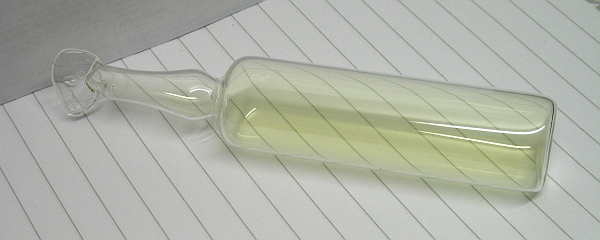
\includegraphics[height=2.9cm]{images/book2/chlorine.jpg}\hspace{0.5em}%
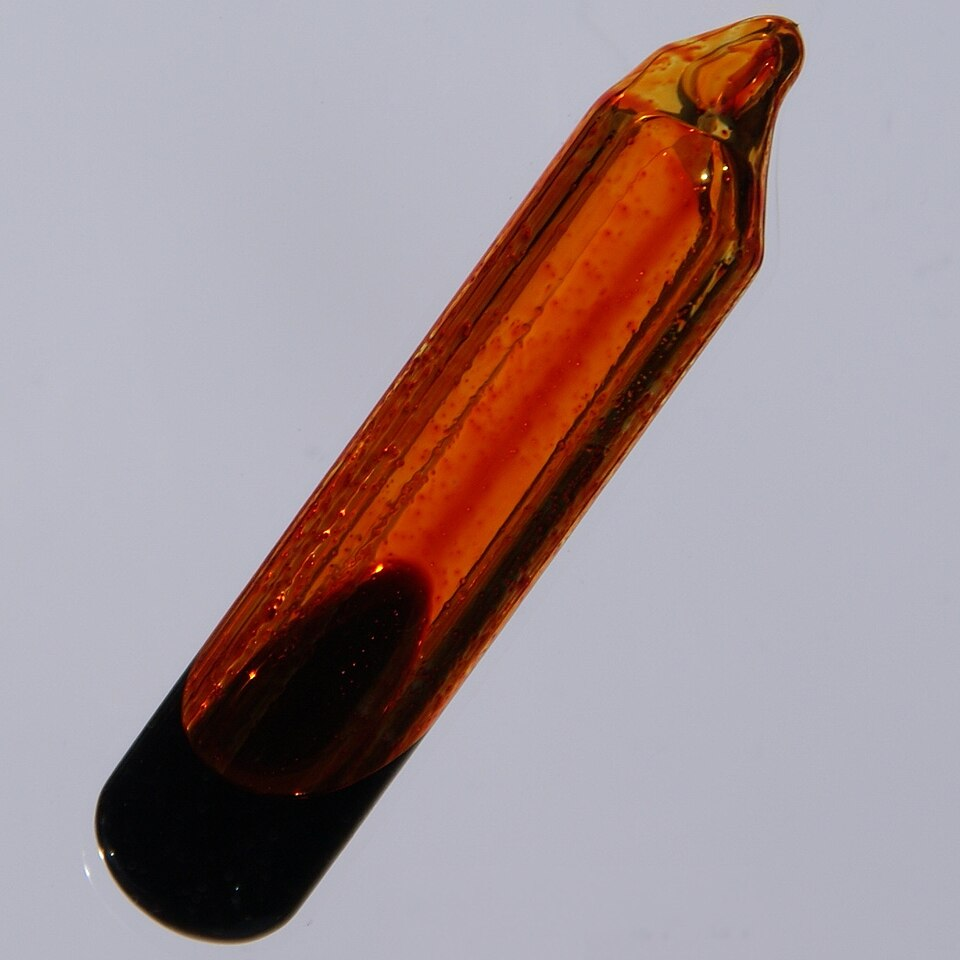
\includegraphics[height=2.9cm]{images/book2/bromine.jpg}\hspace{0.5em}%
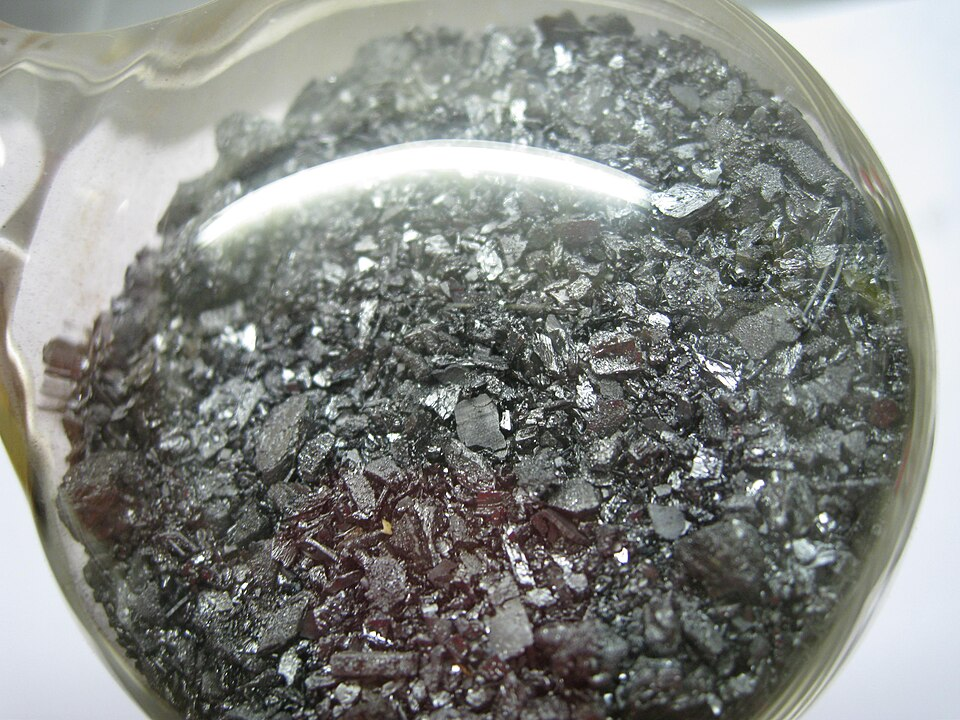
\includegraphics[height=2.9cm]{images/book2/iodine.jpg}

{\small Chlorine, a pale yellow-green gas (W. Oelen, CC BY-SA 3.0);
bromine, a dark red liquid with an orange vapour (Jurii, CC BY 3.0); iodine,
grey-black \omterm{def:b1:crystals-metals:crystal}{crystals} with a metallic lustre (Dnn87, CC BY 3.0). Chlorine and
bromine are sealed in glass ampoules. All Wikimedia Commons.}
\end{omfigure}

\begin{proposition}[Oxidising power of the halogens]\label{prop:b1:p-block-16-18:halogen-oxidising-order}
The \omterm{def:b1:p-block-16-18:halogen}{halogens} are \omterm{def:b1:nernst:couple}{oxidants} whose strength decreases down the group:
$E^\circ(\ce{F2}/\ce{F-}) = 2.89$~V, \ce{Cl2}/\ce{Cl-} 1.36~V,
\ce{Br2}/\ce{Br-} 1.08~V, \ce{I2}/\ce{I-} 0.53~V. Each \omterm{def:b1:p-block-16-18:halogen}{halogen} oxidises the
halide ions below it in the group.
\end{proposition}

\begin{proof}
The values come from the Gibbs energies of formation of the halide ions
(\cref{ch:b1:nernst}). By the gamma rule, \ce{X2} oxidises \ce{Y-} when the
couple \ce{X2}/\ce{X-} lies above \ce{Y2}/\ce{Y-}: for example
\ce{Cl2 + 2Br- -> 2Cl- + Br2}, $\log K = 2(1.36 - 1.08)/0.059 = 9.5$.
Down the group, the atoms grow, their affinity for an extra electron and
the hydration of the smaller halide ions fall, and so does the potential.
\end{proof}
% ledger: dfg:F-_ao, dfg:Cl-_ao, dfg:Br-_ao, dfg:I-_ao

\begin{omfigure}
\begin{tikzpicture}
\begin{axis}[
  ybar, width=0.62\linewidth, height=5.0cm, ymin=0, ymax=3.3,
  symbolic x coords={F,Cl,Br,I}, xtick=data,
  xticklabels={\ce{F2}/\ce{F-}, \ce{Cl2}/\ce{Cl-}, \ce{Br2}/\ce{Br-}, \ce{I2}/\ce{I-}},
  ylabel={$E^\circ$ (V)}, bar width=16pt, nodes near coords,
  every node near coord/.append style={font=\scriptsize},
  tick label style={font=\small}, label style={font=\small}, enlarge x limits=0.2]
\addplot[fill=omThm!40, draw=omThm] coordinates {(F,2.89) (Cl,1.36) (Br,1.08) (I,0.53)};
\end{axis}
\end{tikzpicture}

{\small \omterm{def:b1:nernst:electrode-potential}{Standard potentials} of the halogen--halide couples at
\qty{25}{\celsius}, computed from tabulated Gibbs energies: the oxidising
power falls steadily down the group.}
\end{omfigure}

The hydrogen halides are all acids in water, but \ce{HF} is weak
($\mathrm{p}K_a$ 3.16) while \ce{HCl}, \ce{HBr} and \ce{HI} are strong: the
\ce{H-F} bond is very strong and the small fluoride ion is held in strong
\omterm{def:b1:intermolecular-forces-solvents:hbond}{hydrogen bonds}. Fluorine is the most electronegative element and the
strongest \omterm{def:b1:nernst:couple}{oxidant} of the table; it is obtained only by electrolysis.
Chlorine's \omterm{def:b1:p-block-13-15:oxoacid}{oxoacids} --- hypochlorous \ce{HClO}, chloric \ce{HClO3},
perchloric \ce{HClO4} --- grow stronger with the number of oxygens without
hydrogen, as for all \omterm{def:b1:p-block-13-15:oxoacid}{oxoacids} (\cref{def:b1:p-block-13-15:oxoacid}); their
interplay with chloride and chlorine was mapped in
\cref{ch:b1:e-ph-diagrams}.
% ledger: dfg:HF_ao, dfg:F-_ao

\begin{omfigure}
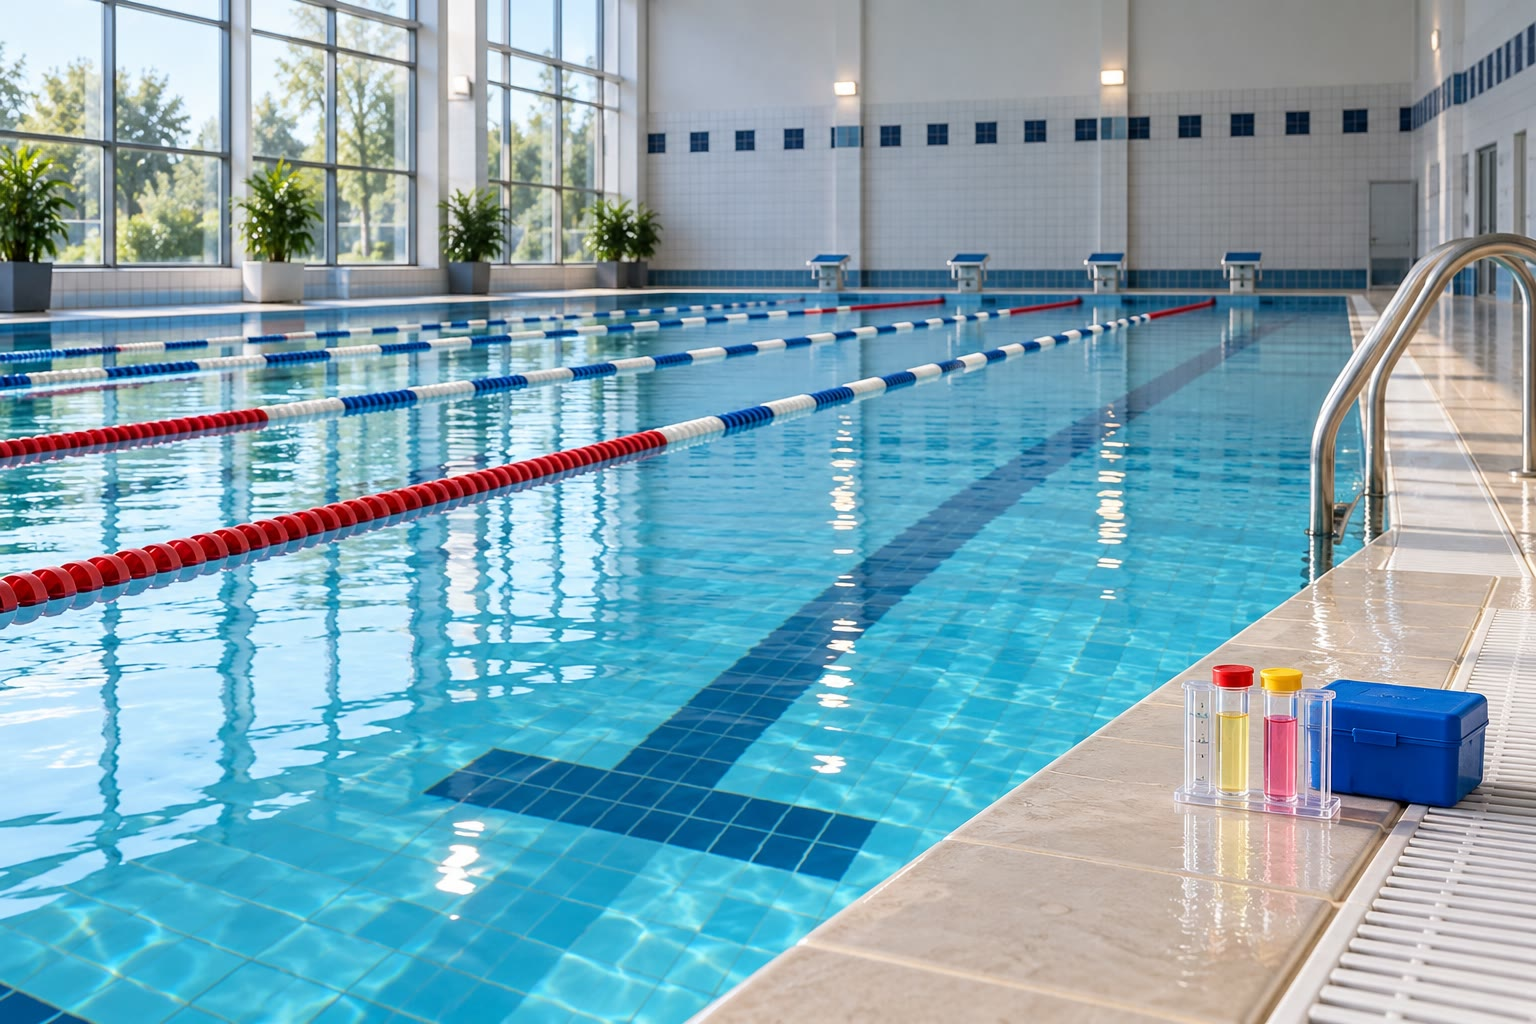
\includegraphics[width=0.55\linewidth]{images/book2/ai/b1-28-swimming-pool.jpg}

{\small A public swimming pool and its water-testing kit: the chlorine
dissolved as hypochlorous acid is checked several times a day.}
\end{omfigure}

\begin{definition}[Interhalogen compounds]\label{def:b1:p-block-16-18:interhalogen}
An \emph{interhalogen compound}\index{interhalogen compound} is a compound
of two different \omterm{def:b1:p-block-16-18:halogen}{halogens}: \ce{ICl}, \ce{BrF3}, \ce{ClF3}, \ce{IF7}. The
larger, less electronegative \omterm{def:b1:p-block-16-18:halogen}{halogen} is the \omterm{def:b1:complexation:complex}{central atom}, with an expanded
octet in \ce{ClF3} and above.
\end{definition}

\begin{inthelab}[Handling the halogens]
Chlorine is toxic and is prepared only in small amounts in a fume
cupboard; bromine burns the skin and its vapour attacks the lungs, and is
used diluted, in a fume cupboard, with gloves and goggles, sodium
thiosulfate solution at hand to destroy spills
(\ce{4Br2 + S2O3^2- + 5H2O -> 8Br- + 2SO4^2- + 10H+}). Iodine is the mildest
of the three, but stains and sublimes; it is kept in a closed bottle.
\end{inthelab}

\section{Noble gases and their compounds}

The noble gases (He, Ne, Ar, Kr, Xe, Rn) have filled valence shells and the
highest ionisation energies of their \omterm{def:b1:periodicity:table}{periods} (\cref{ch:b1:periodicity}).
Long believed inert, the heavier ones, whose outer electrons are less
tightly held, do react with the most electronegative elements: xenon gives
\ce{XeF2}, \ce{XeF4}, \ce{XeF6} and oxides. Their shapes follow the VSEPR
rules with \omterm{def:b1:lewis-resonance-vsepr:lewis}{lone pairs} on xenon.

\begin{example}[Why xenon, and not argon]
The first ionisation energies of the noble gases fall down the group: He
24.59, Ne 21.56, Ar 15.76, Kr 14.00, Xe 12.13, Rn 10.75~eV. That of
dioxygen, \ce{O2 -> O2+ + e-}, is 12.07~eV, almost the same as xenon's. An
\omterm{def:b1:nernst:couple}{oxidant} strong enough to take an electron from \ce{O2}, giving the
dioxygenyl cation \ce{O2+}, should therefore oxidise xenon as well, but not
argon, which holds its electron 3.7~eV more tightly. Xenon does react
with the very strong \omterm{def:b1:nernst:couple}{oxidant} platinum hexafluoride \ce{PtF6}, giving a solid
of overall composition \ce{XePtF6}, and with fluorine itself, which gives
the xenon fluorides of the table below. Radon, easier still to ionise, is
too radioactive for much chemistry to be done on it.
\end{example}
% ledger: ie:He, ie:Ne, ie:Ar, ie:Kr, ie:Xe, ie:Rn, ie:O2, lit:XePtF6

\begin{omfigure}
\begin{tabular}{llll}
\hline
molecule & electron pairs on the \omterm{def:b1:complexation:complex}{central atom} & shape & measured angle \\
\hline
\ce{SO2} & 2 bonding domains + 1 \omterm{def:b1:lewis-resonance-vsepr:lewis}{lone pair} & bent & \ang{119.5} \\
\ce{SF6} & 6 bonding & octahedral & \ang{90} \\
\ce{ClF3} & 3 bonding + 2 \omterm{def:b1:lewis-resonance-vsepr:lewis}{lone pairs} & T-shaped & \ang{87.5} \\
\ce{XeF2} & 2 bonding + 3 \omterm{def:b1:lewis-resonance-vsepr:lewis}{lone pairs} & linear & \ang{180} \\
\ce{XeF4} & 4 bonding + 2 \omterm{def:b1:lewis-resonance-vsepr:lewis}{lone pairs} & square planar & \ang{90} \\
\hline
\end{tabular}

\smallskip
{\small Shapes of some \omterm{def:b1:periodicity:table}{p-block} molecules with expanded octets or \omterm{def:b1:lewis-resonance-vsepr:lewis}{lone pairs}
(measured angles where available). The \omterm{def:b1:lewis-resonance-vsepr:lewis}{lone pairs} of \ce{XeF2} occupy the
three equatorial positions of a trigonal bipyramid, leaving the molecule
linear.}
% ledger: geo:SO2.aOSO, geo:SF6.aFSF, geo:ClF3.aFClF, geo:XeF2.aFXeF
\end{omfigure}

Argon, almost one per cent of air, protects reactive materials in laboratories and
welding; helium, from natural gas, cools superconducting magnets, such as
those of NMR spectrometers (\cref{ch:b1:structure-spectroscopy}).
% ledger: air:Ar

\section{Exercises}

\begin{exercise}[$\star$]\label{exo:b1:p-block-16-18:1}
Give the \omterm{def:b1:nernst:oxidation-number}{oxidation number} of sulfur in \ce{H2S}, \ce{S8}, \ce{SO2},
\ce{SO3^2-}, \ce{SO4^2-}, \ce{S2O3^2-} (average) and \ce{H2S2O7}.
\end{exercise}

\begin{exercise}[$\star$]\label{exo:b1:p-block-16-18:2}
Which of these reactions occur: chlorine with potassium iodide; iodine with
sodium bromide; bromine with sodium chloride; chlorine with sodium bromide?
Write those that do.
\end{exercise}

\begin{exercise}[$\star$]\label{exo:b1:p-block-16-18:3}
Draw the \omterm{def:b1:lewis-resonance-vsepr:lewis}{Lewis structures} of \ce{SO2}, \ce{SO3} and \ce{O3}, with their
\omterm{def:b1:lewis-resonance-vsepr:resonance}{resonance structures}, and give their shapes.
\end{exercise}

\begin{exercise}[$\star$]\label{exo:b1:p-block-16-18:4}
Write the reactions of \ce{SO2} and \ce{SO3} with water and with sodium
hydroxide.
\end{exercise}

\begin{exercise}[$\star\star$]\label{exo:b1:p-block-16-18:5}
Compute the pH of hydrofluoric acid at \qty{0.10}{mol/L} and compare with
hydrochloric acid at the same concentration. Explain the difference.
\end{exercise}

\begin{exercise}[$\star\star$]\label{exo:b1:p-block-16-18:6}
Predict with VSEPR the shapes of \ce{BrF5}, \ce{IF7} (seven \omterm{def:b1:lewis-resonance-vsepr:lewis}{bonding pairs},
pentagonal bipyramid), \ce{ICl4-} and \ce{XeO3}.
\end{exercise}

\begin{exercise}[$\star\star$]\label{exo:b1:p-block-16-18:7}
Compute the constant of \ce{Cl2 + 2I- -> 2Cl- + I2} and say why chlorine
water turns a starch--iodide paper blue.
\end{exercise}

\begin{exercise}[$\star\star$]\label{exo:b1:p-block-16-18:8}
Show that ozone can oxidise iodide ions to iodine and write the reaction in
acid. Why is this used to measure ozone?
\end{exercise}

\begin{exercise}[$\star\star$]\label{exo:b1:p-block-16-18:9}
Concentrated sulfuric acid chars sucrose, \ce{C12H22O11}. Write the
\omterm{def:b1:alcohol-activation:dehydration}{dehydration} to carbon and compute the mass of carbon from \qty{10.0}{g} of
sugar.
\end{exercise}

\begin{exercise}[$\star\star\star$]\label{exo:b1:p-block-16-18:10}
Compute the pH of sulfuric acid at \qty{0.10}{mol/L}, taking the second
acidity into account ($\mathrm{p}K_a = 1.99$). How much does the second
acidity add?
\end{exercise}

\begin{exercise}[$\star\star\star$]\label{exo:b1:p-block-16-18:11}
Using the potentials, explain why fluorine cannot be prepared by oxidising
fluoride with any chemical \omterm{def:b1:nernst:couple}{oxidant} in water, and why it must be made by
electrolysis of a molten fluoride, not of an aqueous solution.
\end{exercise}

\begin{exercise}[$\star\star\star$]\label{exo:b1:p-block-16-18:12}
Iodine is only slightly soluble in water but dissolves in potassium iodide
solution as the triiodide ion \ce{I3-}. Using the Gibbs energies of
\ce{I2(aq)} ($\Delta_f G^\circ = \qty{16.40}{kJ/mol}$), \ce{I-} ($-51.57$)
and \ce{I3-} ($-51.4$), compute the constant of \ce{I2 + I- <=> I3-}.
\end{exercise}

\section{Problem: One Tonne of Sulfur}

\begin{problem}[{Weekend problem --- burning sulfur, the catalytic
oxidation of sulfur dioxide, absorption and oleum, the second acidity of
sulfuric acid, and the mass of acid made from one tonne of sulfur}]
\label{pb:b1:p-block-16-18:1}
A sulfuric acid plant burns sulfur recovered from natural gas. Molar masses
(\unit{g/mol}): S 32.1, \ce{O2} 32.0, \ce{SO2} 64.1, \ce{SO3} 80.1,
\ce{H2SO4} 98.1, \ce{H2O} 18.0; air contains \qty{21}{\percent} of
\ce{O2} by volume; $\mathrm{p}K_a(\ce{HSO4-}) = 1.99$; $R =
\qty{8.314}{J/(K.mol)}$.

\medskip
\noindent\textbf{Part I --- Burning sulfur.}
\begin{enumerate}
  \item Give the \omterm{def:b1:nernst:oxidation-number}{oxidation number} of S in S, \ce{SO2}, \ce{SO3} and
        \ce{H2SO4}.
  \item Write the combustion of sulfur.
  \item Draw the \omterm{def:b1:lewis-resonance-vsepr:lewis}{Lewis structure} of \ce{SO2} and predict its shape.
  \item Compute the amount of sulfur in one tonne.
  \item Compute the volume of air (\qty{25}{\celsius}, \qty{1}{bar}) for
        the combustion alone.
  \item Why is the gas from the burner cooled before the converter?
\end{enumerate}

\medskip
\noindent\textbf{Part II --- Catalytic oxidation.}
\begin{enumerate}[resume]
  \item Write the oxidation of \ce{SO2} to \ce{SO3}.
  \item Its constant at \qty{25}{\celsius} is about $10^{24.8}$. Why is a
        \omterm{def:b1:elementary-steps:catalyst}{catalyst} nevertheless needed?
  \item What is the role of vanadium(V) oxide, in the language of
        \cref{ch:b1:elementary-steps}?
  \item Draw the shape of \ce{SO3}.
  \item Why is excess air used?
  \item What fraction of \ce{SO2} is lost if the conversion is
        \qty{99.7}{\percent}?
\end{enumerate}

\medskip
\noindent\textbf{Part III --- Absorption.}
\begin{enumerate}[resume]
  \item Write the absorption of \ce{SO3} in sulfuric acid.
  \item Why is \ce{SO3} not absorbed directly in water?
  \item Write the dilution of oleum.
  \item Write the overall equation of the process.
  \item Compute the mass of water consumed per tonne of sulfur.
  \item Why must the acid be poured into water and never the reverse?
\end{enumerate}

\medskip
\noindent\textbf{Part IV --- The acid.}
\begin{enumerate}[resume]
  \item Compute the pH of a \qty{0.050}{mol/L} solution of sulfuric acid
        with the second acidity taken into account.
  \item Compute the mass of sulfuric acid for a \qty{99.5}{\percent}
        overall \omterm{def:b1:extent-q-and-k:fractional-extent}{yield}.
  \item The world produced about \qty{84}{Mt} of sulfur in 2025. What
        mass of sulfuric acid would it give if all were converted?
  \item State the mass of sulfuric acid obtainable from one tonne of
        sulfur (complete conversion).
\end{enumerate}
\end{problem}
